\chapter{Background} \label{ch:background}

This chapter introduces the biological and neuromorphic ideas used in the model. The aim is not to reproduce bat auditory biology in full anatomical detail. Instead, the background is organised around the computations needed for active acoustic localisation: extracting timing, level, and spectral cues from an echo; converting them into neural population codes; and decoding those populations into distance, azimuth, and elevation estimates.

\section{Echolocation as Active Localisation}

Echolocating bats localise objects by emitting an acoustic call and analysing the returning echo. This is an active sensing problem rather than passive listening: the animal knows approximately what signal it emitted, when it emitted it, and how that signal should change after reflection from a target. The returning echo therefore carries cues for distance, azimuth, and elevation. These cues are not independent; the same echo amplitude, frequency content, and arrival time are affected by target range, head geometry, ear shape, and environmental noise. The biological problem is to separate these interacting effects quickly enough to guide flight.

Bats are useful inspiration because their sensing problem is close to a radar problem but is solved by a compact, event-driven nervous system. Many echolocating species use frequency-modulated (FM) sweeps, sometimes with constant-frequency (CF) components, as shown in Figure~\ref{fig:bat_call_redraft}. The FM sweep is important for this project because it produces a broadband time-frequency pattern: a delayed echo can be matched against an internal copy of the emitted sweep, while the echo spectrum can also carry elevation information.

\begin{figure}[H]
    \centering
    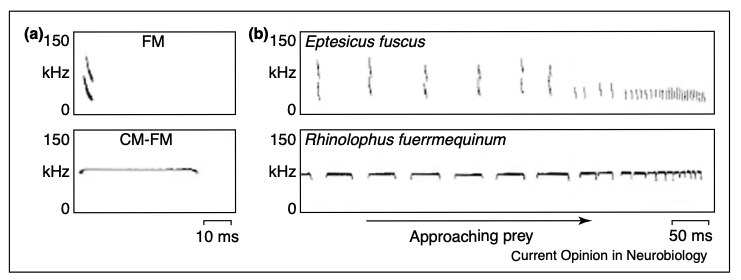
\includegraphics[width=0.86\linewidth]{2_Background/background_figures/Auditory_localisation/bat_call.png}
    \caption{Echolocation signal structures. (a) Examples of FM and CF components used by echolocating bats. (b) Signal sequences produced while pursuing prey; pulse rate increases and call duration decreases as the bat approaches the target \cite{MossANeurobiologyBats}.}
    \label{fig:bat_call_redraft}
\end{figure}

\section{Auditory Cues for 3D Position}

\subsection{Distance}

In passive listening, absolute range is difficult because the original source intensity is unknown. Active echolocation provides a stronger cue: time-of-flight (ToF). If an emitted call reflects from a target and returns after delay $\Delta t$, the target range is approximately
\begin{equation}
    r = \frac{c\Delta t}{2},
    \label{eq:tof_distance_redraft}
\end{equation}
where $c$ is the speed of sound and the factor of two accounts for the outward and return path. This is the main distance cue used in the model. Echo amplitude also decreases with propagation distance, but intensity is less reliable because it depends on target reflectivity, call intensity, ear direction, and environmental conditions.

The biological complication is that the brain does not contain a simple digital clock. It must represent delay using neural signals. In bats, delay-sensitive neurons respond selectively to particular pulse-echo delays, so range can be represented as activity over a bank of candidate delays rather than as a single stopwatch value \cite{Suzuki2017AcuityBats}.

\subsection{Azimuth}

Azimuth is the horizontal angle of the target. It is mainly estimated using binaural differences: the difference between the signals at the two ears. The first cue is interaural time difference (ITD), the arrival-time difference between ears. In a simple straight-line approximation,
\begin{equation}
    \theta = \arcsin\left(\frac{c\,\mathrm{ITD}}{d}\right),
    \label{eq:itd_azimuth_redraft}
\end{equation}
where $\theta$ is azimuth and $d$ is the interaural distance. This ignores diffraction around the head, but it captures the key computational idea: a timing difference maps monotonically to horizontal angle over the frontal region.

The second cue is interaural level difference (ILD), the amplitude difference between the two ears. At high frequencies the head casts an acoustic shadow, reducing sound level at the far ear. Because bat calls are high frequency, ILD can be a strong azimuth cue, although its reliability depends on head size, frequency, and source direction. The classical duplex theory states that ITD is most useful at low frequencies and ILD at high frequencies \cite{Rayleigh1907Direction}; for this project the important point is simpler: timing and level comparisons provide complementary azimuth evidence.

ITD alone is ambiguous. A cone of directions can share the same interaural delay, as shown in Figure~\ref{fig:azimuth_cues_redraft}. This is one reason why elevation-dependent spectral cues and multiple cue pathways are needed.

\begin{figure}[H]
    \centering
    \begin{subfigure}[t]{0.5\textwidth}
        \textbf{\large A}\\[0.5ex]
        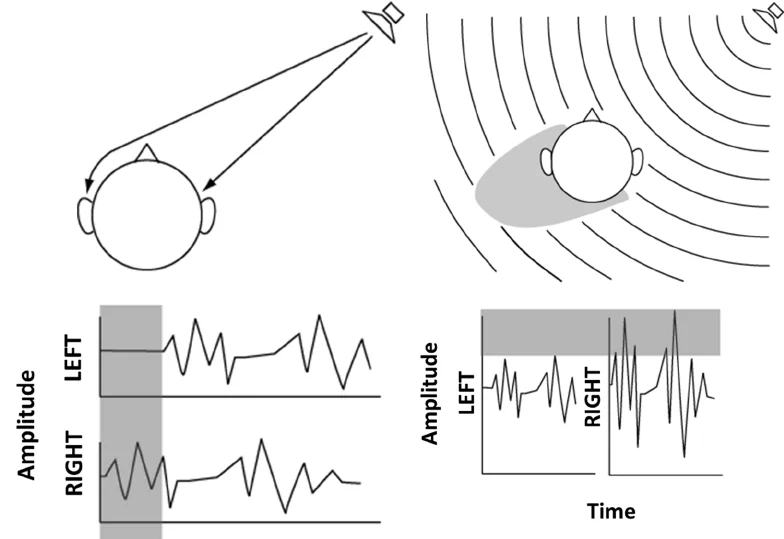
\includegraphics[height=4.8cm]{2_Background/background_figures/Auditory_localisation/itd_ild.png}
        \caption{}
    \end{subfigure}
    \hspace{0.1cm}
    \begin{subfigure}[t]{0.32\textwidth}
        \textbf{\large B}\\[0.5ex]
        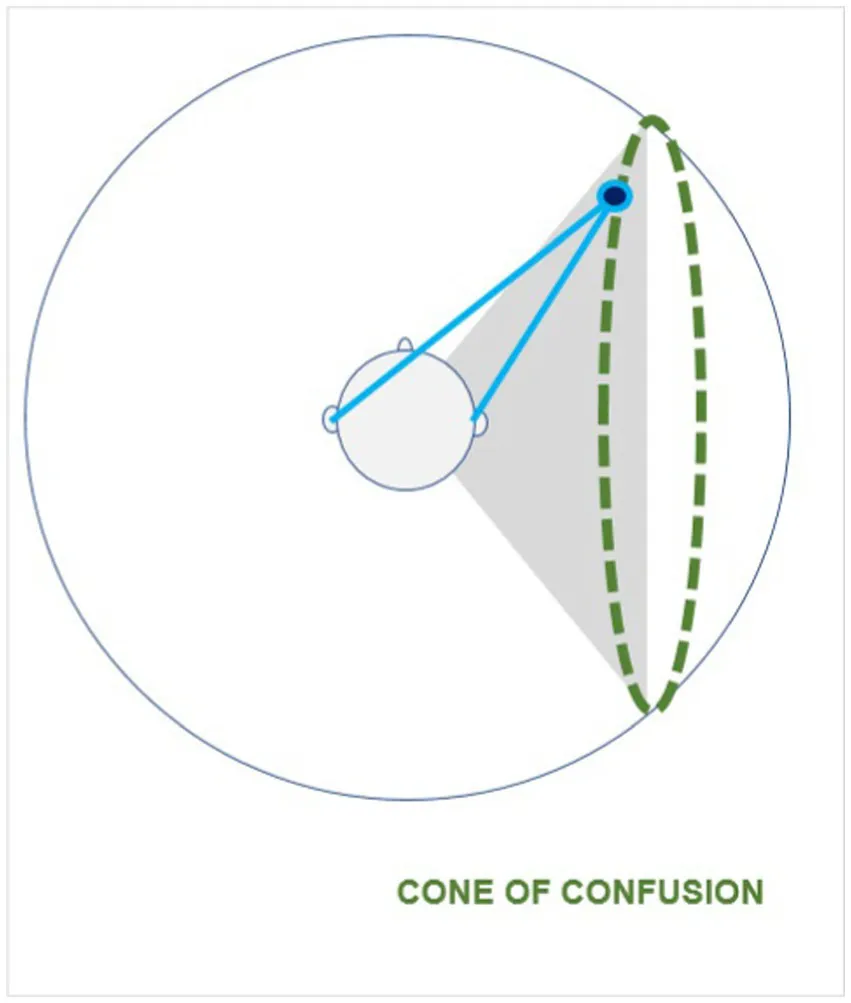
\includegraphics[height=4.8cm]{2_Background/background_figures/Auditory_localisation/cone.png}
        \caption{}
    \end{subfigure}
    \caption{A: ITD and ILD cues. B: cone of confusion for constant ITD \cite{Sun2015DynamicListeners,Carlini2024AuditoryReview}.}
    \label{fig:azimuth_cues_redraft}
\end{figure}

\subsection{Elevation}

Elevation is the vertical angle of the target. Because the left and right ears are mostly separated horizontally, binaural timing and level differences are weaker vertical cues. Instead, elevation is strongly linked to spectral filtering by the outer ear, or pinna. A sound arriving from different vertical angles reflects from the ridges of the pinna in different ways, producing direction-dependent peaks and notches in the spectrum. The full direction-dependent filtering of the head, torso, and outer ears is called the head-related transfer function (HRTF) \cite{Carlini2024AuditoryReview,Zonooz2019SpectralElevation}.

For this project, the relevant abstraction is a comb-filter cue: the received signal is combined with a delayed copy of itself, producing spectral notches whose frequencies depend on the delay. If the filtered signal is
\begin{equation}
    y(t) = x(t) + g x(t-\tau),
\end{equation}
then the magnitude response is
\begin{equation}
    |H(f)| = \frac{\sqrt{1+g^2+2g\cos(2\pi f\tau)}}{1+g}.
    \label{eq:comb_filter_background_redraft}
\end{equation}
Changing $\tau$ moves the notch pattern. This is not a complete HRTF model, but it creates the same kind of computational problem: elevation must be inferred from a frequency-dependent spectral shape rather than from a simple time delay. Figure~\ref{fig:elevation_cues_redraft} shows the biological pinna mechanism and the kind of elevation-dependent HRTF map that motivates this abstraction.

\begin{figure}[H]
    \centering
    \begin{subfigure}[t]{0.45\textwidth}
        \textbf{\large A}\\[0.5ex]
        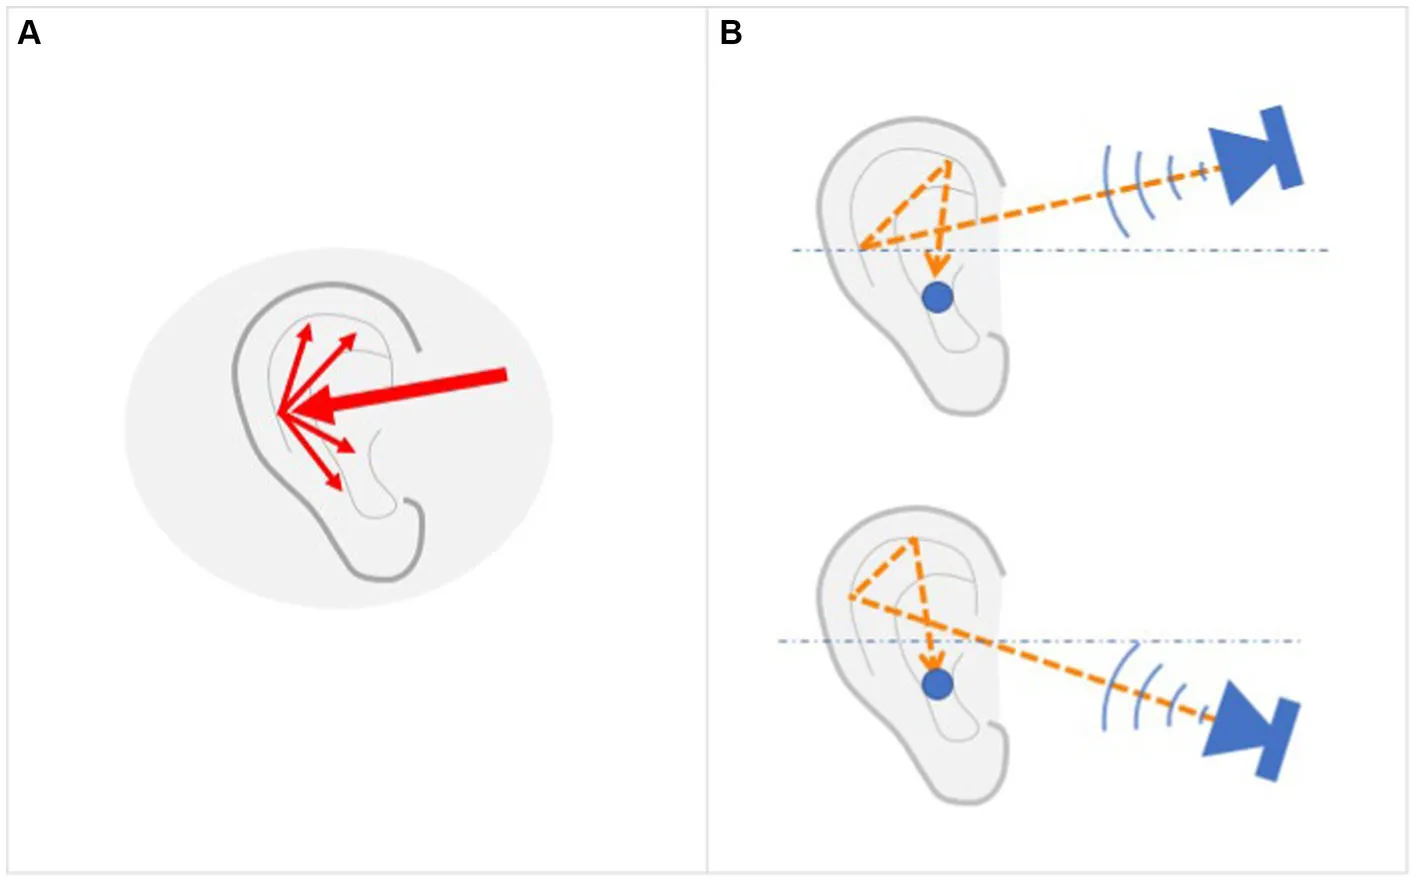
\includegraphics[height=3.8cm]{2_Background/background_figures/Auditory_localisation/pinna_1.png}
        \caption{}
    \end{subfigure}
    \hspace{0.1cm}
    \begin{subfigure}[t]{0.45\textwidth}
        \textbf{\large B}\\[0.5ex]
        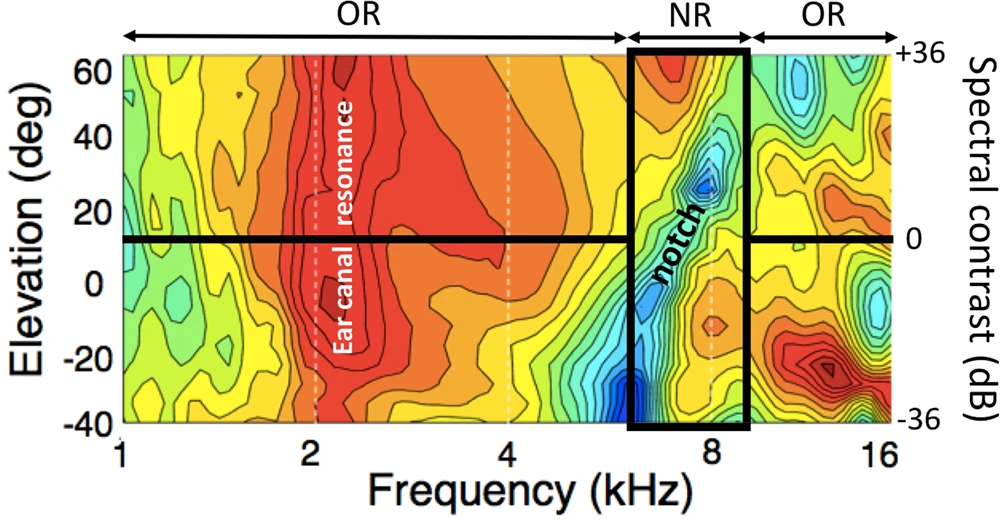
\includegraphics[height=3.8cm]{2_Background/background_figures/Auditory_localisation/pinna_map.png}
        \caption{}
    \end{subfigure}
    \caption{A: pinna-based HRTF mechanism. B: measured elevation-dependent HRTF structure, with red indicating high gain and blue indicating low gain \cite{Carlini2024AuditoryReview,Zonooz2019SpectralElevation}.}
    \label{fig:elevation_cues_redraft}
\end{figure}

\section{Biological Auditory Pathways as Computation}
\label{sec:biology}

The bat auditory system is highly specialised, but the model in this report uses a functional abstraction rather than a full anatomical simulation. Figure~\ref{fig:overall_pathway_redraft} is the key biological scaffold. The left side shows the ascending auditory pathway, where acoustic signals are transformed into neural representations. The right side shows descending and vocalisation pathways, which are simplified here into an emitted call and a corollary discharge. A corollary discharge is an internal copy of a self-generated motor command or expected sensory signal; in echolocation it provides a reference against which the returning echo can be compared.

\begin{figure}[H]
    \centering
    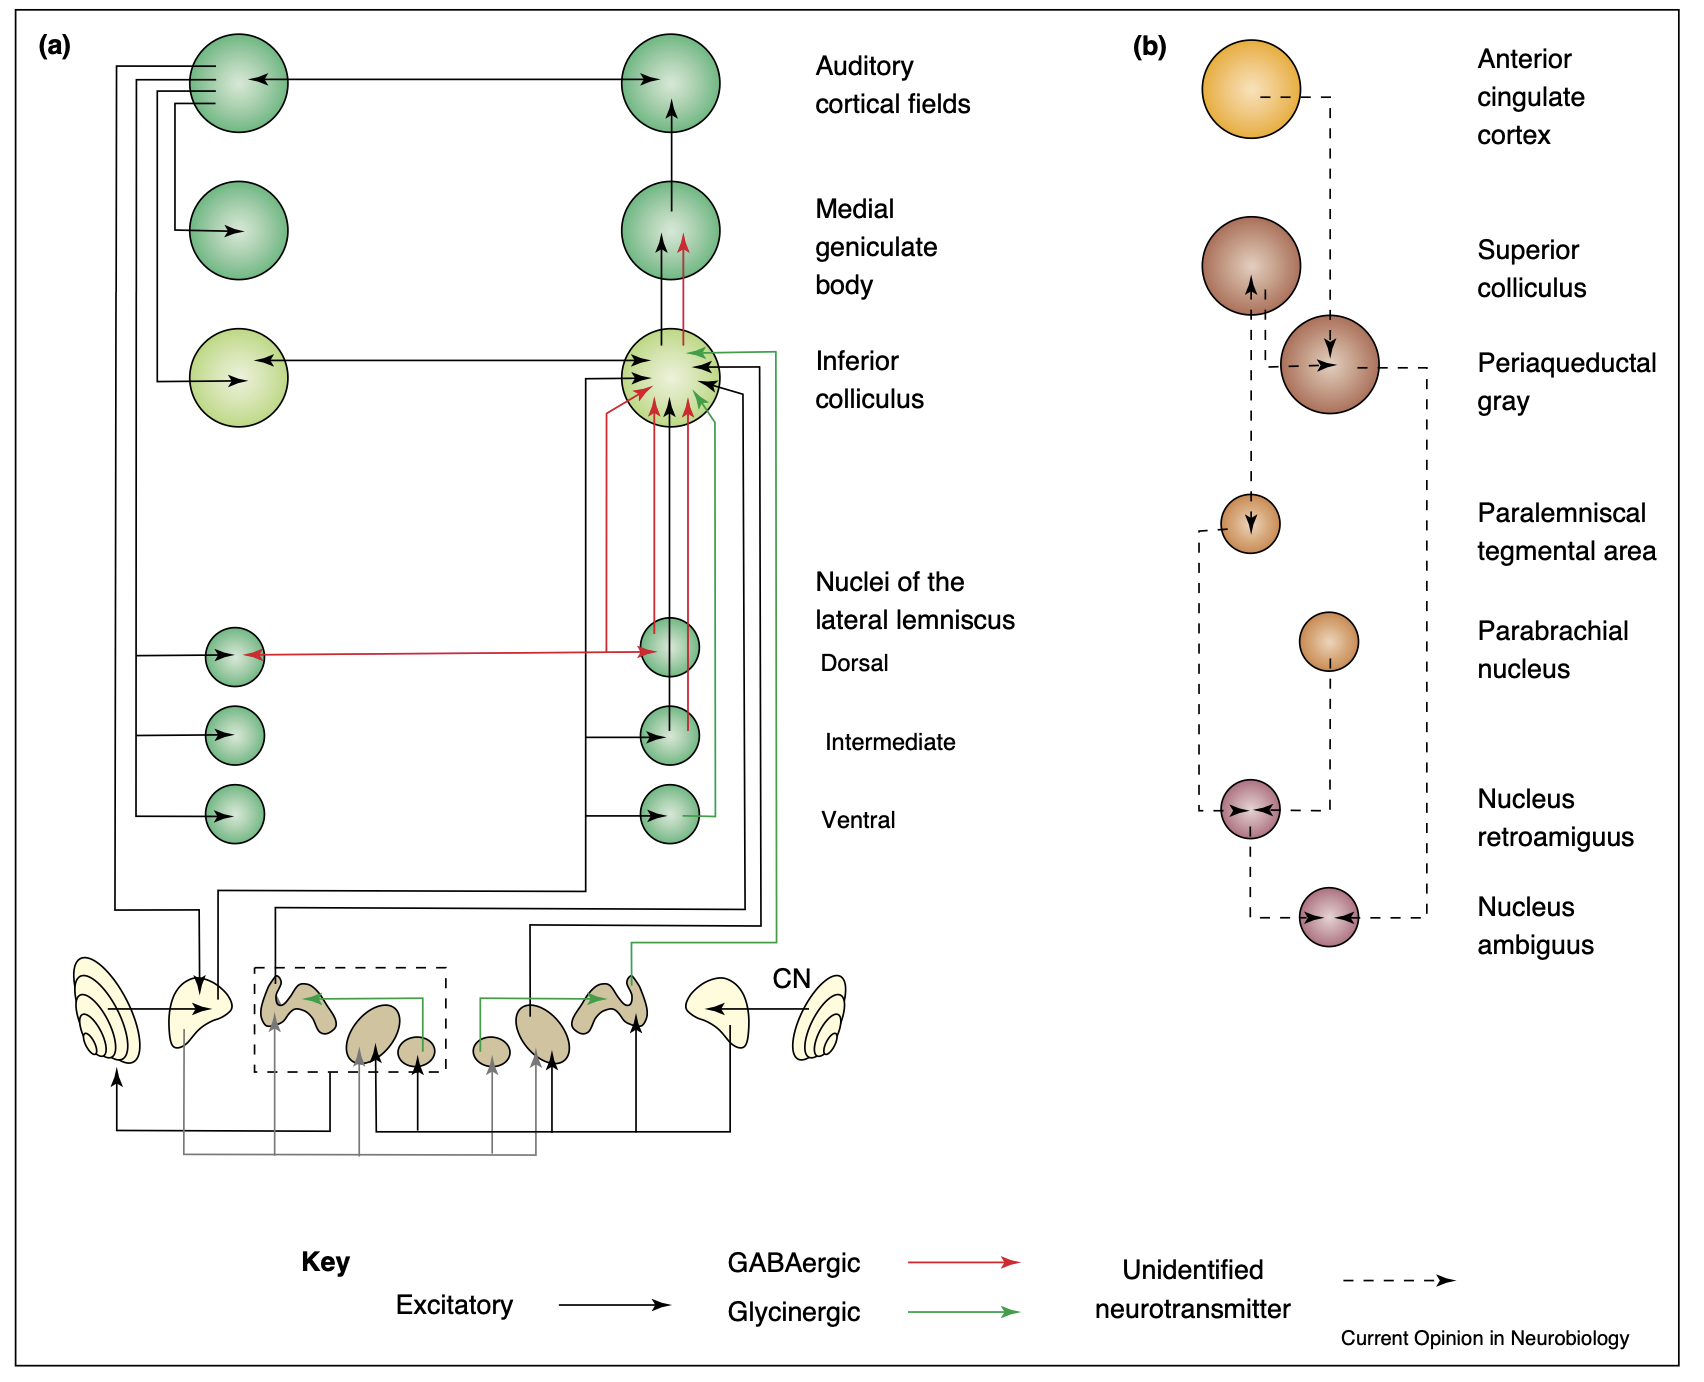
\includegraphics[width=\textwidth]{2_Background/background_figures/biology/overall_brain.png}
    \caption{Major ascending auditory connections and descending vocalisation circuitry in bat echolocation \cite{MossANeurobiologyBats}. In this project the detailed vocalisation pathway is simplified to an emitted call and a corollary-discharge copy, while the ascending pathway motivates the cochlea, distance, azimuth, elevation, and SC readout modules.}
    \label{fig:overall_pathway_redraft}
\end{figure}

The modelling principle is that each biological region is treated as a computing block. A neuron can be viewed, loosely, as an analogue switch with memory: it integrates weighted inputs through synapses, compares its internal state with a threshold, and emits a spike when the threshold is crossed. Inhibitory neurons act like suppressive switches, reducing activity elsewhere. This logic-gate analogy is imperfect because real neurons are noisy, adaptive, and chemical, but it is useful for engineering: networks of excitatory and inhibitory spiking units can implement filtering, comparison, coincidence detection, and population decoding.

\subsection{Cochlea and Tonotopic Encoding}

The cochlea converts air-pressure waveforms into neural activity. It is tonotopic, meaning different positions along the cochlea respond preferentially to different frequencies. High frequencies peak near the base, lower frequencies further along the basilar membrane. This spatial frequency decomposition is shown in Figure~\ref{fig:cochlea_redraft}. The output is not a continuous spectrogram but a set of neural signals from frequency-selective channels.

\begin{figure}[H]
    \centering
    \begin{subfigure}[t]{0.45\textwidth}
        \textbf{\large A}\\[0.5ex]
        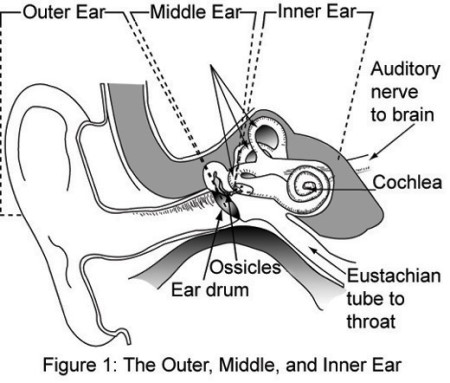
\includegraphics[height=3.8cm]{2_Background/background_figures/biology/cochlea.png}
        \caption{}
    \end{subfigure}
    \hspace{0.1cm}
    \begin{subfigure}[t]{0.45\textwidth}
        \textbf{\large B}\\[0.5ex]
        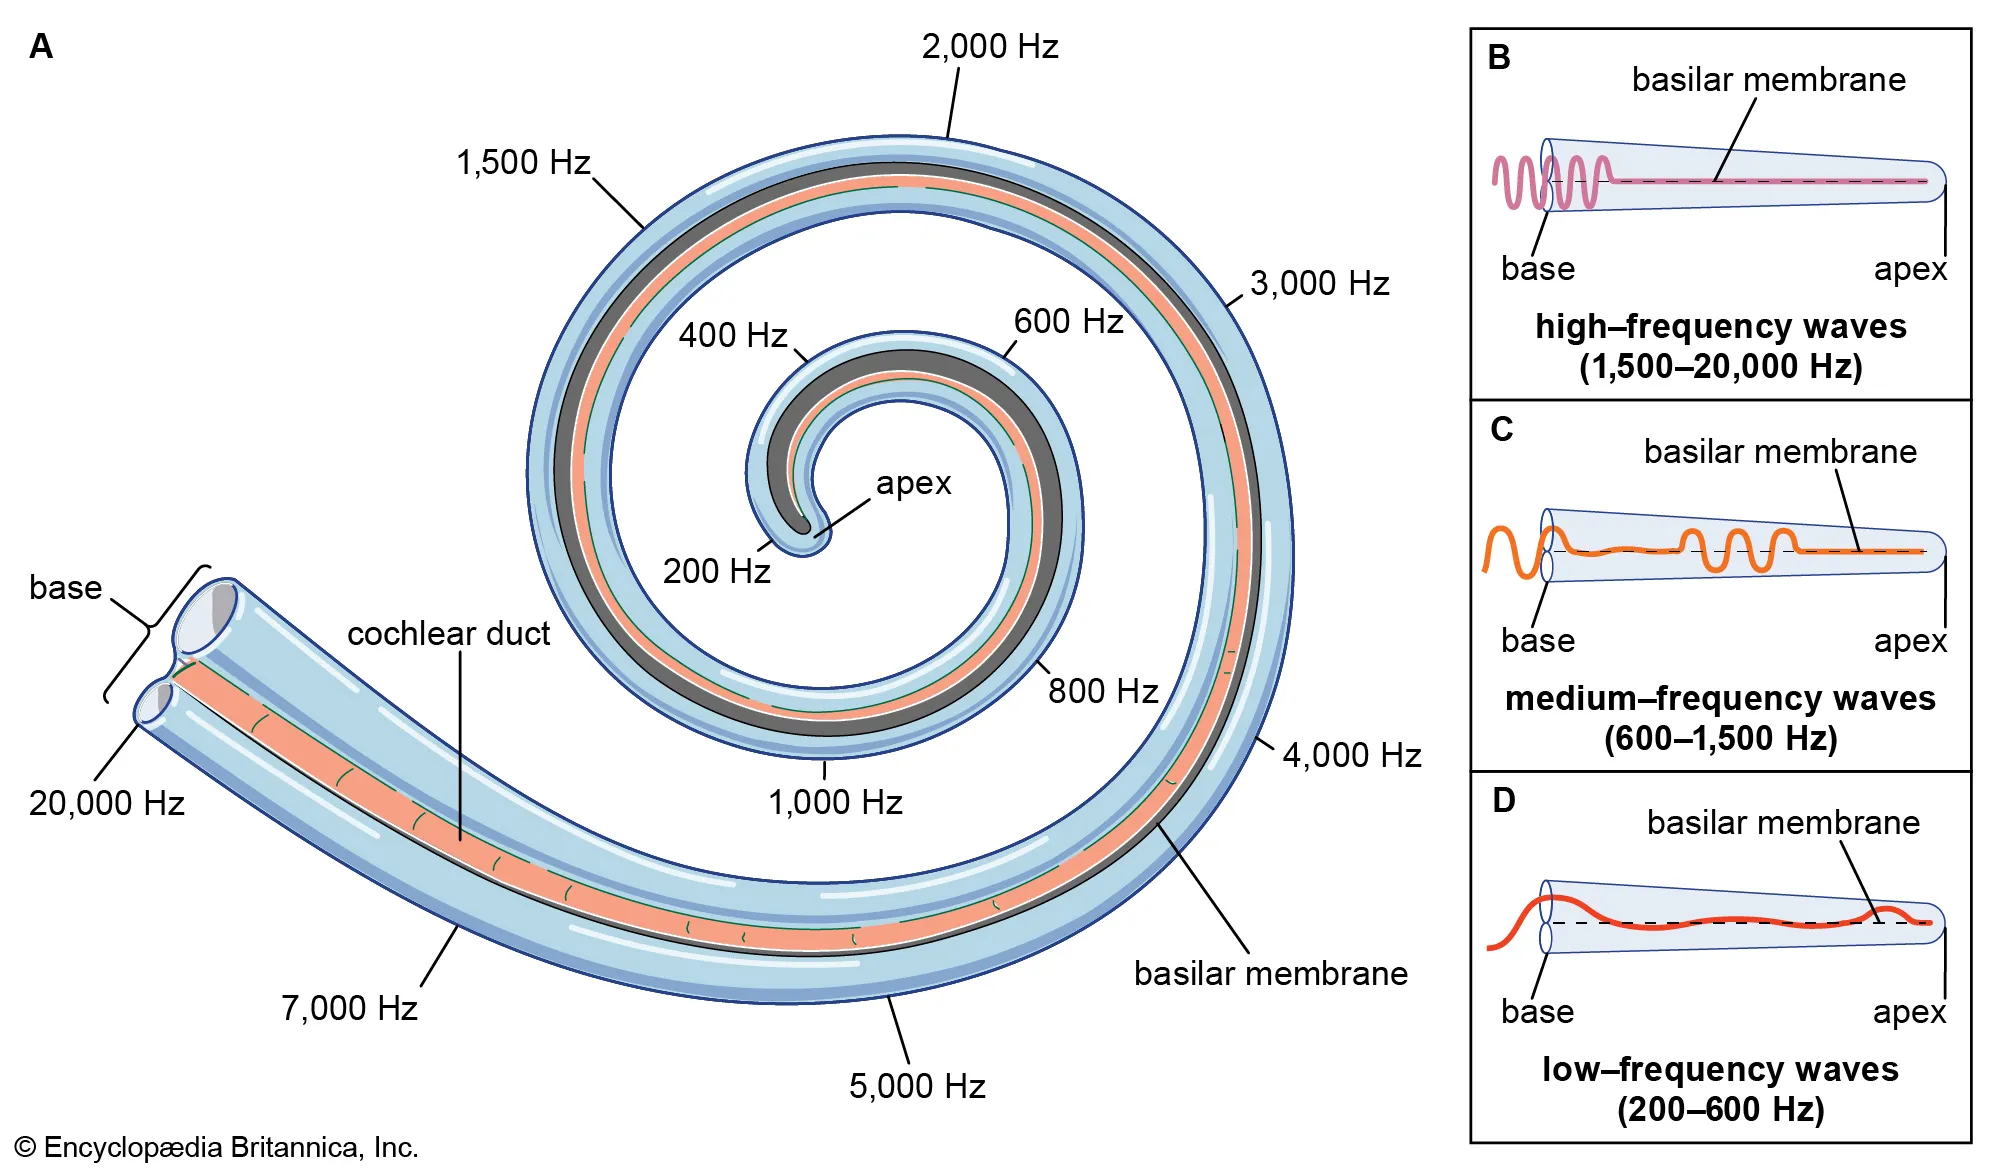
\includegraphics[height=3.8cm]{2_Background/background_figures/biology/spiral.png}
        \caption{}
    \end{subfigure}
    \caption{A: outer, middle, and inner ear. B: tonotopic frequency organisation along the cochlea \cite{CochleaStudy.com,HumanBritannica}.}
    \label{fig:cochlea_redraft}
\end{figure}

In the model, this motivates a cochlear filterbank followed by spike encoding. The exact biophysics of basilar-membrane fluid mechanics are not simulated. Instead, the cochlea is abstracted as a bank of frequency-selective filters whose outputs are converted into cochlear spike rasters. This retains the computational features needed later: frequency selectivity, timing, and sparse events.

\subsection{Cochlear Nuclei, Onset Cleaning, and Pathway Splitting}

After the cochlea, auditory nerve fibres project to the cochlear nuclei (CN). The CN can be understood as an early router and feature extractor. Ventral cochlear nucleus (VCN) neurons are specialised for preserving precise timing and onset information. This matters for distance and ITD, where sub-millisecond timing errors can shift the inferred position. The dorsal cochlear nucleus (DCN) is more closely associated with spectral processing and is therefore relevant to elevation cues.

The biological details are richer than this abstraction, but the functional split is the important part for the report. The model uses VCN/VNLL-inspired onset processing to clean the cochlear spike raster before distance and azimuth coincidence detection. For elevation, the model uses a DCN-like spectral population that compares the observed frequency profile with expected comb-filter templates.

\subsection{Midbrain and Cortical Population Maps}

The inferior colliculus (IC) and auditory cortex (AC) contain neurons sensitive to combinations of timing, frequency, and binaural cues. For distance, FM-FM delay-tuned neurons respond strongly when an emitted-call component and an echo component arrive with a particular delay. For azimuth, Jeffress-style delay-line models provide a useful abstraction: signals from the two ears are passed through different internal delays, and coincidence neurons respond when the delayed inputs align \cite{Jeffress1948ALocalization}. For elevation, spectral shape can be mapped into a population of candidate elevations.

The key modelling choice is therefore to represent each coordinate as a population code. A population code stores a value as a pattern of activity across many neurons, each tuned to a candidate coordinate. A single neuron might represent ``about 3 ms delay'' or ``about +20 degrees elevation'', but the final estimate is decoded from the whole activity pattern. This matters because biological precision can exceed the spacing of individual neurons: a smooth population peak can be decoded between the centres of neighbouring neurons.

\subsection{The SC as a Readout Abstraction}

The superior colliculus (SC) is involved in spatial orienting and sensorimotor maps. In this project it is treated as the final coordinate-readout stage rather than as a detailed motor-control model. The detailed descending vocalisation pathway is collapsed into two model components: the emitted call and the corollary-discharge copy used by the distance pathway. This is a deliberate simplification. It keeps the model focused on localisation while preserving the core active-sensing idea: the brain compares an internally available reference with the returning echo.

\section{Coincidence Detection and Population Codes}
\label{sec:coincidence_background}

Coincidence detection is central to the distance and azimuth pathways, so it is worth defining carefully. A coincidence detector is a neuron or circuit that fires strongly only when two inputs arrive close together in time. If one input arrives too early, its membrane voltage decays before the second arrives. If it arrives too late, the same happens in reverse. When the inputs are aligned, their effects add and can cross the firing threshold.

This turns timing comparison into a spatial neural code. Suppose the brain has an internal copy of the emitted call and a bank of internal delay lines. Each delay line shifts the copy by a different candidate delay. The echo is compared with each delayed copy. The neuron whose internal delay best matches the true echo delay receives near-simultaneous inputs and therefore has the strongest response. ``Maximal firing'' in this context means the largest spike count or membrane response within the candidate population, not a mysterious property of a single neuron. Figure~\ref{fig:delay_line_coincidence_population_redraft} gives the corresponding delay-line population example.

\begin{figure}[H]
    \centering
    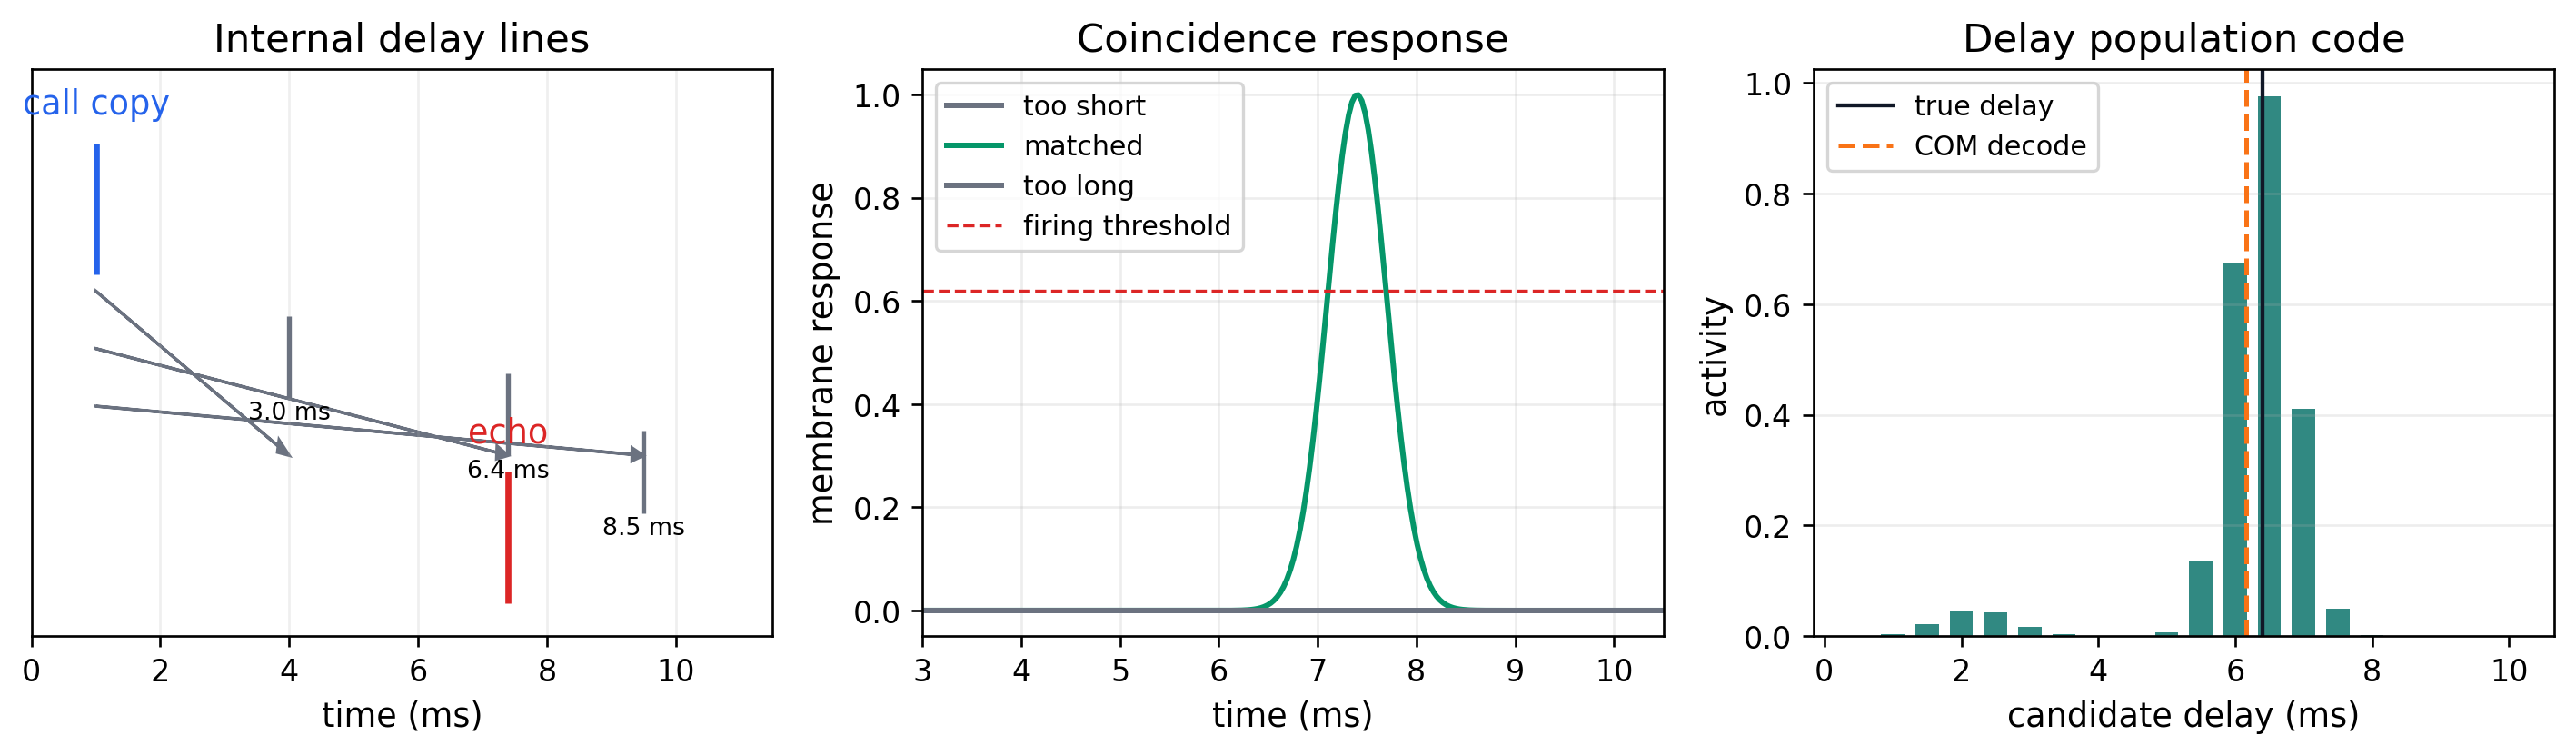
\includegraphics[width=\textwidth]{2_Background/background_figures/neuromorphic/delay_line_coincidence_population.png}
    \caption{Delay-line coincidence detection. An internal call copy is passed through candidate delays and compared with the echo. Matched timing produces the largest membrane response, creating a delay population that can be decoded by centre of mass (COM) or an SC-style readout.}
    \label{fig:delay_line_coincidence_population_redraft}
\end{figure}

This population-code view connects the Suga and Simmons perspectives on bat ranging. Suga-style delay-tuned neurons support the idea of discrete biological delay channels, while behavioural hyperacuity suggests that bats can achieve finer precision than a simple nearest-neuron readout would imply \cite{Suzuki2017AcuityBats}. A natural compromise is population decoding: use the full pattern of responses across delay-tuned neurons rather than only the index of the largest one. This is why the model later uses centre-of-mass decoding and SC-style continuous attractor readouts.

Continuous attractor neural networks (CANNs) also fit here. A CANN is a recurrent population in which local excitation and broader inhibition can stabilise a bump of activity. In this report, CANNs are not treated as the main source of intelligence. They are used as one possible SC-like readout for a population code: the upstream pathway produces an activity bump, and the recurrent readout can smooth or stabilise it before decoding.

Rate coding is the other important abstraction. A fully spiking population produces individual spike trains, but many downstream computations can use average spike count or firing rate over a short window. This is still biologically meaningful: rate is a summary of spiking activity, not a replacement for it. In the model, this justifies using explicit spike rasters where timing matters, and rate-coded population vectors where the relevant information is the strength of activity across candidate coordinates.

\section{Spiking Computation}

Spiking neural networks (SNNs) use event-like spikes rather than continuously valued activations. In the model, a spike is a binary event at a timestep, effectively a discrete Kronecker-delta impulse rather than a continuous analogue value. Figure~\ref{fig:lif_spike_population_encoding_redraft} shows the basic spike-generation and population-code ideas. A standard leaky integrate-and-fire (LIF) neuron integrates input current into a membrane state. The membrane leaks over time, and when it crosses a threshold the neuron emits a spike and resets. In discrete time this can be written as
\begin{equation}
    v[t] = \beta v[t-1] + I[t] - S[t]V_{\mathrm{th}},
    \qquad
    S[t] = \mathbb{I}\left[v[t]\geq V_{\mathrm{th}}\right],
    \label{eq:lif_background_redraft}
\end{equation}
where $v[t]$ is membrane voltage, $I[t]$ is input, $\beta$ is the leak factor, $V_{\mathrm{th}}$ is threshold, and $S[t]$ is the emitted spike. This is the basic circuit element used throughout the report.

\begin{figure}[H]
    \centering
    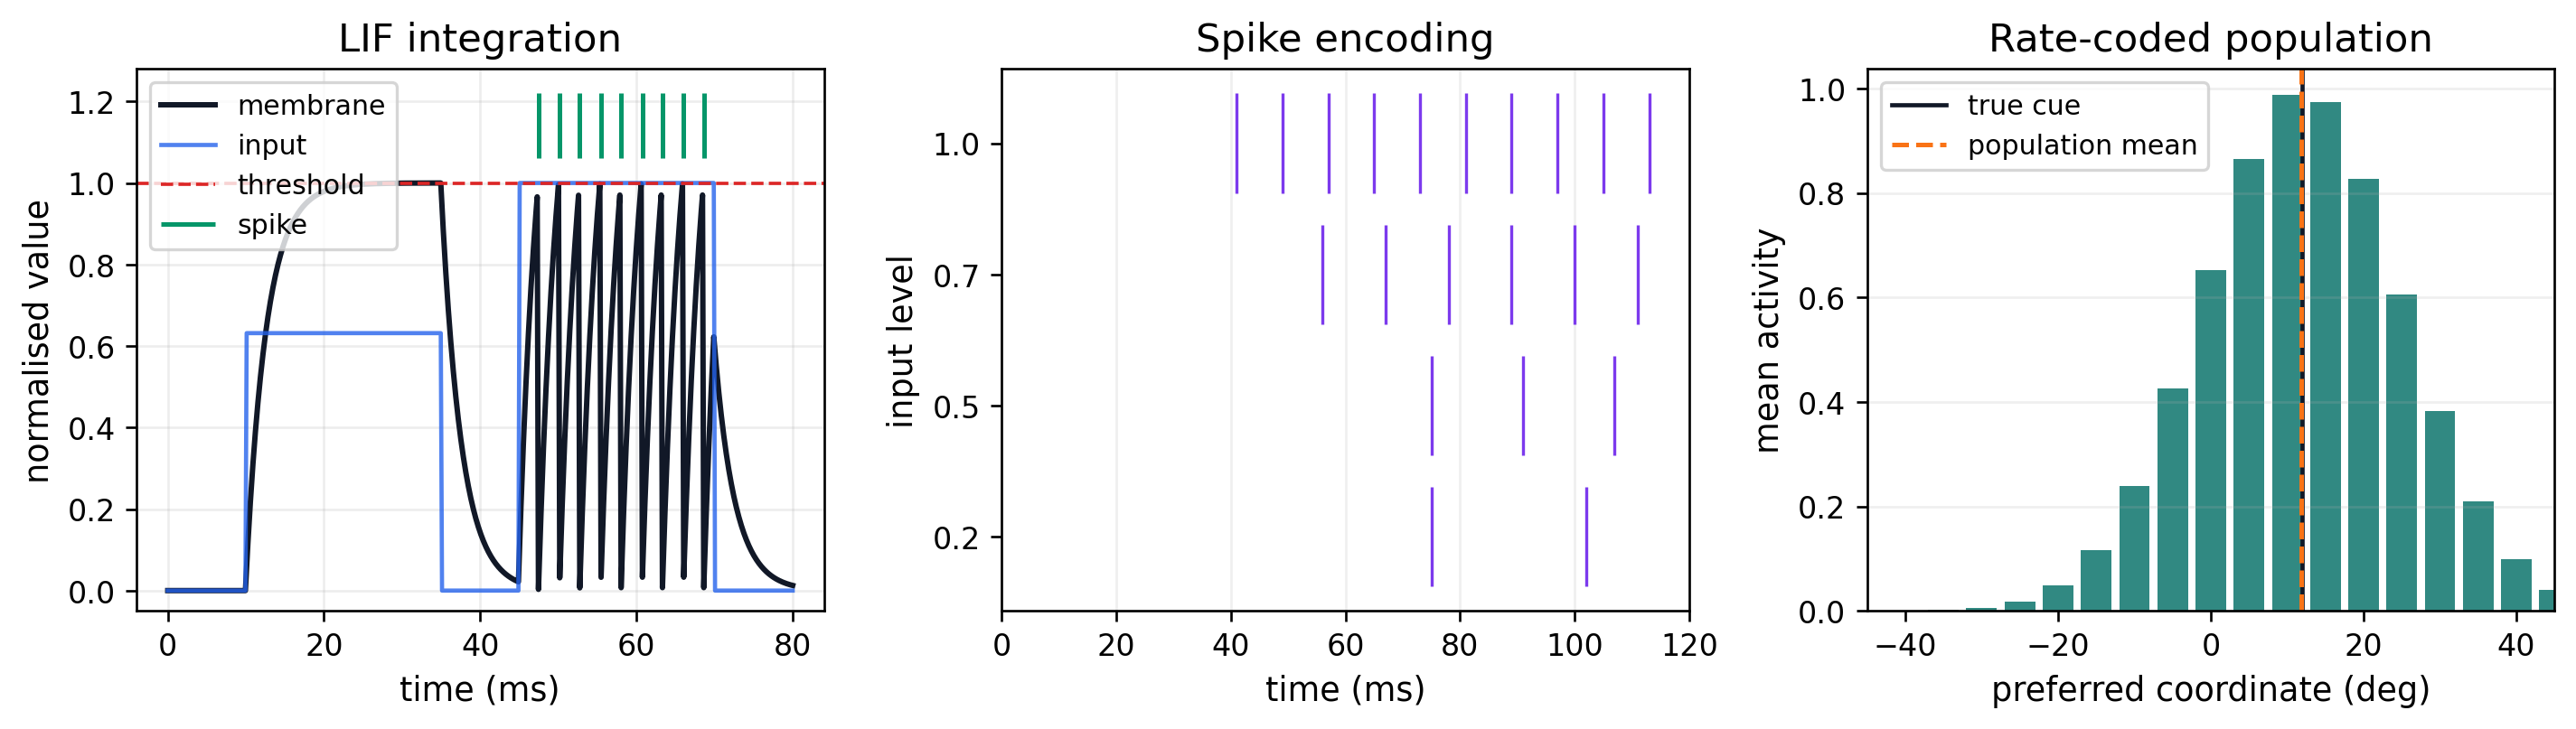
\includegraphics[width=\textwidth]{2_Background/background_figures/neuromorphic/lif_spike_population_encoding.png}
    \caption{Spiking computation primitives. A LIF neuron integrates input until threshold crossing, stronger inputs can be encoded by earlier or denser spike trains, and a population of neurons can represent a continuous coordinate through average activity.}
    \label{fig:lif_spike_population_encoding_redraft}
\end{figure}

The engineering attraction of spikes is that computation can be event-driven. Event-driven processing means that downstream computation is triggered by discrete events, such as incoming spikes, rather than by updating every unit with dense synchronous operations at every timestep. If no spikes arrive, little needs to be updated. Neuromorphic hardware exploits this sparsity by implementing large numbers of spiking neurons and synapses with asynchronous communication; large digital neuromorphic chips such as TrueNorth demonstrated million-neuron spiking systems with low-power event-driven operation \cite{Merolla2014AInterface}. This does not automatically mean every SNN is efficient, but it motivates building models whose data representation and computations could be mapped to neuromorphic hardware.

Modern trainable SNNs often use surrogate gradients. The spike function is non-differentiable, so during backpropagation its derivative is replaced with a smooth approximation. Forward simulation still uses spikes, while the backward pass uses a differentiable surrogate. This allows SNNs to be trained using deep-learning tools while retaining spiking dynamics \cite{Eshraghian2023TRAININGLEARNING}. In this project, the final trainable model uses SNN readouts to test whether the biologically structured pathway features are more useful than raw waveform or cochlear-raster inputs.

\section{Current Models and Project Gap}

Existing sound-localisation models span conventional signal processing, probabilistic localisation, artificial neural networks, and neuromorphic systems. Reviews of auditory localisation identify ITD, ILD, and HRTF cues as the main physical basis for human and animal spatial hearing \cite{Carlini2024AuditoryReview}. Neuromorphic sound-source localisation systems often focus on one or two binaural cues, particularly ITD and ILD, and many are motivated by the biological MSO/LSO structure of the auditory brainstem \cite{Danneville2024ASystems}. Earlier computational models also used Bayesian or probabilistic cue integration for binaural localisation \cite{Li2003ALocalization,Willert2006ALocalization}.

The gap addressed here is narrower and more specific. This project is not simply applying an SNN to audio. It asks whether a biologically structured, modular echolocation pathway can produce useful intermediate representations for 3D active localisation. The model therefore includes an emitted FM call, echo simulation, cochlear spike encoding, separate distance/azimuth/elevation pathways, population-code readouts, and a final trainable SNN fusion stage. The results can then distinguish between two explanations: either the final SNN succeeds because any trainable network could solve the task, or it succeeds because the biologically inspired pathways provide useful features.

This framing also explains the level of biological simplification used in the modelling chapter. Detailed anatomical realism is not the objective. The objective is to identify biological computations that are useful and implementable: tonotopic filtering, onset preservation, coincidence detection, spectral template matching, lateral inhibition, population coding, recurrent readout stabilisation, and trainable spike-based fusion.
